\section{Le LHC: \emph{Large Hadron Collider}}\label{chapter-LHC-section-LHC}
Le Grand Collisionneur de Hadrons~\cite{LHC_paper1,LHC_paper2,LHC_paper3} (LHC, \emph{Large Hadron Collider}) est le plus grand et le plus puissant accélérateur de particules au monde.
Son tracé ainsi que ceux du \emph{Booster}, du PS et du SPS sont illustrés sur la figure~\ref{fig-CERN_map}.
Le LHC est installé dans le même tunnel que le LEP, il s'agit donc d'un accélérateur circulaire de \SI{27}{\kilo\meter} de circonférence, situé entre \num{50} et \SI{100}{\meter} sous la frontière franco-suisse.
\par Le LHC permet de réaliser des collisions proton-proton, proton-ion lourd et ion lourd-ion lourd.
Les collisions d'ions lourds permettent de reproduire les conditions des premiers instants de l'Univers après le \emph{Big Bang} et sont principalement étudiée par l'expérience ALICE, une des quatre expériences du LHC présentées dans la section~\ref{chapter-LHC-section-LHC-subsec-experiments}.
Dans tous les cas, deux faisceaux de particules sont accélérés en sens inverses.
Seules les collisions de protons sont considérées dans cette thèse.
\subsection{Exploitation du LHC}\label{chapter-LHC-section-LHC-subsec-LHC_runs}
Le fonctionnement du LHC peut être divisé en plusieurs périodes ou \emph{Runs}.
Chaque \emph{Run} du LHC présente différentes caractéristiques, en particulier l'énergie dans le centre de masse des collisions.
Le tableau~\ref{tab-LHC_runs} résume les différents \emph{Runs} du LHC, passés et à venir.
Chaque \emph{Run} est lui-même divisé par année civile, des arrêts techniques étant faits en période hivernale.
Enfin, une année civile est subdivisée en plusieurs périodes (A, B, C, etc.) entre lesquelles les conditions expérimentales peuvent varier, comme la nature des particules entrant en collision.
\begin{table}[h]
\centering
\begin{tabular}{cccc}
\toprule
Run & Période & Énergie dans le centre de masse & Luminosité\\
\midrule
I & 2011-2012 & 7 à \SI{8}{\TeV} & \SI{30}{\femto\barn^{-1}} \\
II & 2016-2018 & \SI{13}{\TeV} & \SI{190}{\femto\barn^{-1}} \\
III & 2021-2024 & 13 à \SI{14}{\TeV} & \SI{350}{\femto\barn^{-1}}? \\
IV & 2027-2030 & \SI{14}{\TeV} & \multirow{2}{*}{\SI{3000}{\femto\barn^{-1}}?}\\
V & 2032-2034 & \SI{14}{\TeV} & \\
\bottomrule
\end{tabular}
\caption[Runs du LHC.]{Runs du LHC avec les énergies dans le centre de masse et les luminosités correspondantes~\cite{LHC_commissioning}. La luminosité est présentée dans la section~\ref{chapter-LHC-section-LHC-subsec-lumi}.}
\label{tab-LHC_runs}
\end{table}
\subsection{Accélération de protons}\label{chapter-LHC-section-LHC-subsec-pp_acceleration}
Les protons sont obtenus par ionisation de dihydrogène, directement issu d'une bouteille.
Les protons sont alors progressivement accélérés à travers différentes installations du CERN, illustrées sur la figure~\ref{fig-chapter-LHC-section-CERN-CERN_Accelerator-Complex}, menant les protons à des niveaux d'énergie de plus en plus hauts avant de pouvoir être injectés dans le LHC~\cite{LHC_paper3}:
\begin{itemize}
\item l'accélérateur linéaire 2 (LINAC~2)\footnote{Le LINAC~2 est remplacé pour le Run~III du LHC par le LINAC~4.} permet d'accélérer les protons à une énergie de \SI{50}{\MeV};
\item le \emph{Booster}, premier élément circulaire, amène les protons à \SI{1.4}{\GeV};
\item le PS permet d'atteindre \SI{25}{\GeV};
\item le SPS, dernier élément avant le LHC, accélère les protons jusqu'à \SI{450}{\GeV}.
\end{itemize}
Le LHC accélère alors les protons jusqu'à \SI{6.5}{\TeV} lors du Run~II et ira jusqu'à \SI{7}{\TeV} lors du Run~III, permettant de réaliser des collisions avec des énergies dans le centre de masse de \num{13} et \SI{14}{\TeV}, respectivement.
\par Le gain en énergie des particules, \ie\ l'accélération colinéaire aux faisceaux, se fait dans le LHC à l'aide de 16 cavités radiofréquences, 8 par faisceau.
Ces cavités créent un champ électrique oscillant.
Cette technique présente l'avantage d'accélérer les particules différemment selon leurs positions respectives, ce qui permet de les conserver en plusieurs paquets dont l'intérêt est développé dans la section suivante.
\par Afin de maintenir les particules dans le tube circulaire du LHC, leur trajectoire est courbée, \ie\ qu'une accélération orthogonale aux faisceaux est appliquée.
Cette courbure s'obtient grâce à un champ magnétique de \SI{8.33}{\tesla} généré par 1232 aimants dipolaires supraconducteurs répartis tout au long des \SI{27}{\kilo\meter} du LHC et refroidis à l'hélium superfluide à \SI{1.8}{\kelvin}.
\subsection{Collisions de protons}\label{chapter-LHC-section-LHC-subsec-pp_collisions}
\subsubsection{Structure du proton}
\begin{wrapfigure}{R}{8cm}
\centering
\begin{fmffile}{proton_structure}\fmfstraight
\begin{fmfchar*}(50,30)
  \fmfleft{in1,in2,i1,i2,i3}
  \fmfright{on1,on2,o1,o2,o3}
  \fmf{phantom}{in1,vn1,in2}
  \fmf{phantom,tension=3}{vn1,vn2}
  \fmf{phantom}{on1,vn2,on2}
  \fmf{phantom}{i1,v11,v12,v13,v14,o1}
  \fmf{phantom}{i2,v21,v22,v23,v24,o2}
  \fmf{phantom}{i3,v31,v32,v33,v34,o3}
  \fmffreeze
  \fmf{fermion}{i1,v11,v12,v14,o1}
  \fmf{fermion}{i2,v21,v23,o2}
  \fmf{fermion}{i3,v32,o3}
  \fmf{fermion,left}{vn1,vn2,vn1}
  \fmf{gluon}{v21,v32}
  \fmf{gluon}{v12,v23}
  \fmf{gluon}{v11,vn1}
  \fmf{gluon}{vn2,v14}
  \fmfdot{v21,v32,v23,v12,v11,vn1,vn2,v14}
  \fmflabel{\quarku}{i1}
  \fmflabel{\quarku}{i2}
  \fmflabel{\quarkd}{i3}
  \fmflabel{\quarku}{o1}
  \fmflabel{\quarku}{o2}
  \fmflabel{\quarkd}{o3}
\end{fmfchar*}
\end{fmffile}
\vspace{\baselineskip}
\caption{Diagramme de Feynman de la propagation d'un proton avec apparition d'une paire \quark\antiquark.}
\label{fig-proton_mer_quarks_fmf}
\end{wrapfigure}
Les protons ne sont pas des particules fondamentales, ils possèdent une sous-structure.
En tant que baryons, les protons sont donc des hadrons dont la composition moyenne est de trois quarks, en l'occurrence deux \emph{up} et un \emph{down}.
Cependant, ces quarks échangent des gluons virtuels par l'intermédiaire de l'interaction forte.
Ces gluons peuvent se matérialiser en paires \quark\antiquark, comme illustré sur la figure~\ref{fig-proton_mer_quarks_fmf}.
Au sein des protons, d'autres partons que les trois quarks~\quarku, \quarku\ et~\quarkd\ dits \og de valence \fg{} peuvent donc être présents.
Ces particules additionnelles forment la \og mer \fg{} dans laquelle se trouvent ainsi des gluons, des antiquarks et des quarks de saveurs lourdes.
\par Chacun des constituants du proton porte une fraction $x$ de l'énergie totale du proton.
La probabilité pour qu'un parton $i$ du proton porte une fraction $x_i$ de l'énergie peut être décrite à l'aide des fonctions de densité partoniques (PDF, \emph{Parton Distribution Functions}).
Ces fonctions sont obtenues par ajustement des données expérimentales~\cite{Gao_2018,Ball_2015} et sont représentées sur la figure~\ref{fig-proton_PDFs}.
Les partons de la mer portent généralement une faible fraction de l'énergie.
La fraction d'énergie la plus probable portée par un quark de valence est de \num{10} à \SI{20}{\%} selon l'échelle d'énergie.
L'ensemble des quarks de valence porte ainsi \num{30} à \SI{60}{\%} seulement de l'énergie totale du proton.
Dans le cas du proton, les quarks de valence~\quarku\ portent environ deux fois plus d'énergie que les quarks de valence~\quarkd, ce qui est cohérent avec la structure moyenne (\quarku\quarku\quarkd) du proton.
\begin{figure}[h]
\centering
\subcaptionbox{Pour $\mu^2 = \SI{10}{\GeV^2}$.\label{subfig-proton_PDF_100_GeV2}}[.45\textwidth]
{\begin{tikzpicture}
\node[anchor=south west,inner sep=0] at (0,0) {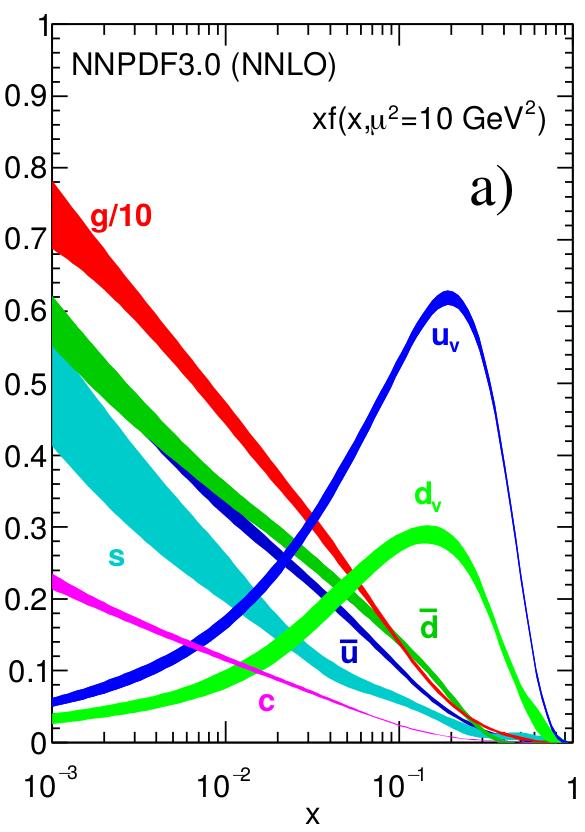
\includegraphics[width=5cm]{\PhDthesisdir/plots_and_images/from_PDG_booklet_2018/parton_pdf_100_GeV2.png}};

% masks
\fill [white] (0,0) rectangle (5,.75);
\fill [white] (0,0) rectangle (.425,7);
\fill [white] (.6,6.7) -- (.6,6) -- (4,5) -- (4.7,5) -- (4.7,6.7);

% X axis
\foreach \pos/\val in {-3/e-3,-2/e-2,-1/e-1,0/1}{
\draw ({4.9+(4.9-.45)*(\pos)/(3)}, .4) node {\footnotesize \num{\val}\vphantom{ÀQg}};
}
\draw (2.7, .2) node {\normalsize $x$};

% Y axis
\foreach \val in {0,0.1,0.2,0.3,0.4,0.5,0.6,0.7,0.8,0.9,1}{
\draw (.5, {.75+\val*(6.9-.75)}) node [left] {\footnotesize \num{\val}};
}

\draw (.5, 6.5) node [right] {\footnotesize NNPDF3.0 (NNLO)};
\draw (4.9,6) node [left] {\scriptsize $x \, f(x, \mu^2=\SI{10}{\GeV^2})$};

\end{tikzpicture}
}
\hfill
\subcaptionbox{Pour $\mu^2 = \SI{e4}{\GeV^2}$.\label{subfig-proton_PDF_10000_GeV2}}[.45\textwidth]
{\begin{tikzpicture}
\node[anchor=south west,inner sep=0] at (-.05,0) {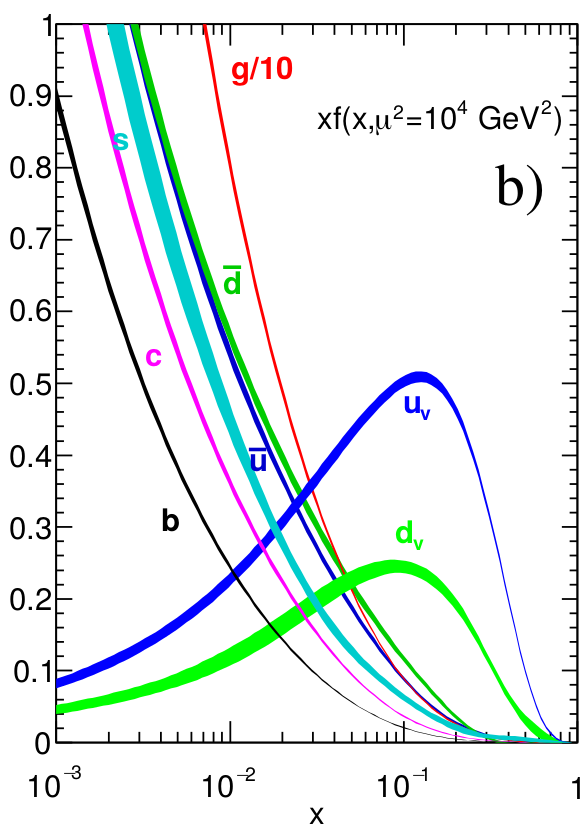
\includegraphics[width=5cm]{\PhDthesisdir/plots_and_images/from_PDG_booklet_2020/parton_pdf_10000_GeV2.png}};

% masks
\fill [white] (0,0) rectangle (5,.75);
\fill [white] (0,0) rectangle (.425,7);
\fill [white] (2.6,6.3) -- (2.6,5.9) -- (4.1,5.2) -- (4.7,5.2) -- (4.7,5.8) -- (4.8,6) -- (4.8,6.2) -- (4.7,6.3);

% X axis
\foreach \pos/\val in {-3/e-3,-2/e-2,-1/e-1,0/1}{
\draw ({4.9+(4.9-.45)*(\pos)/(3)}, .4) node {\footnotesize \num{\val}\vphantom{ÀQg}};
}
\draw (2.7, .2) node {\normalsize $x$};

% Y axis
\foreach \val in {0,0.1,0.2,0.3,0.4,0.5,0.6,0.7,0.8,0.9,1}{
\draw (.5, {.75+\val*(6.9-.75)}) node [left] {\footnotesize \num{\val}};
}

\draw (4.9,6) node [left] {\scriptsize $x \, f(x, \mu^2=\SI{e4}{\GeV^2})$};

\end{tikzpicture}
}
\caption[Fonctions de densité partoniques.]{Fonctions de densité partoniques (PDF, \emph{Parton Distribution Functions}) à différentes échelles d'énergie $\mu$ obtenues au NNLO NNPDF3.0~\cite{NNPDF30} avec $g_s(m_{\Zboson}^2)=\num{0.118}$~\cite{PDG_booklet_2018}. Les bandes tracées correspondent aux PDF $f$, avec incertitude, multipliées la fraction d'impulsion $x$, où $f$ peut être les quarks~\quarku\ et~\quarkd\ de valence ($\quarku_v$, $\quarkd_v$) ou les gluons (\gluon), quarks et antiquarks de la mer (\antiquarku, \antiquarkd, $\quarks\simeq\antiquarks$, $\quarkc=\antiquarkc$, $\quarkb=\antiquarkb$).}
\label{fig-proton_PDFs}
\end{figure}
\par Lorsque deux protons entrent en collision, se sont donc des constituants de ces protons qui interagissent.
Or, le constituant du premier proton ne porte pas forcément une fraction d'énergie $x$ identique à celle que porte le constituant du second proton.
Ainsi, bien que les impulsions des deux protons soient opposées l'une à l'autre, \ie\ que le référentiel du centre de masse des protons coïncide avec le référentiel du détecteur, ceci n'est pas vrai pour les partons impliqués dans la collision.
Lors des collisions de protons, seule l'impulsion totale dans le plan transverse aux faisceaux est donc nulle et l'impulsion selon l'axe des faisceaux est inconnue.
De plus, l'énergie dans le centre de masse des protons n'est pas totalement utilisée dans la collision.
Une collision de partons à \SI{13}{\TeV} est ainsi peu probable au LHC, toutefois ces collisions de protons permettent de balayer une large gamme d'énergies effectives de collision, ce qui est favorable aux recherches de nouvelles particules.
\subsubsection{Faisceaux et paquets de protons}
La dimension spatiale des protons, de l'ordre du femtomètre (\SI{e-15}{\meter}) ne permet pas de les faire se collisionner un à un de manière efficace.
Au LHC, deux faisceaux de protons sont ainsi accélérés, chacun dans un sens.
Afin de ne pas avoir des collisions en permanence, ce qui rendrait impossible une exploitation des signaux dans les détecteurs, les protons des faisceaux sont regroupés par paquets.
Ces paquets sont espacés temporellement de \SI{25}{\nano\second} lors du Run~II, laissant aux instruments de détection un laps de temps suffisant afin de distinguer deux collisions successives.
\par La formation et le maintient de ces paquets est rendue possible par l'utilisation des cavités radiofréquence.
Elles produisent un champ électrique dont la norme est plus importante au niveau des queues des paquets qu'à leurs têtes.
Alors, les protons \og en queue de peloton \fg{} sont plus accélérés que les protons en tête et ils les rattrapent.
\par Dans chacun des deux faisceaux du LHC, 2808 paquets sont ainsi formés.
Avant les premières collisions, un paquet comporte \num{1.15e11} protons.
Les paquets font environ \SI{30}{\centi\meter} de long.
Lorsqu'ils circulent dans le LHC, leur diamètre est de l'ordre du millimètre mais au niveau des points de collisions, un ensemble de champs magnétique réduit ce diamètre à \SI{16}{\micro\meter}.
\par Le passage des \num{1.15e11} protons d'un paquet d'un faisceau du LHC à travers la surface de \SI{16}{\micro\meter} de diamètre, combiné au passage d'un paquet de l'autre faisceau, permet d'obtenir des collisions dures entre protons.
Il s'agit de collisions dans lesquelles les constituants des protons interagissent et créent de nouvelles particules par conservation de l'énergie.
Les faisceaux du LHC sont stables une dizaine d'heures, pendant lesquelles des collisions surviennent 40 millions de fois par seconde.
La luminosité permet de rendre compte de la quantité de collisions réalisées.
\subsection{Luminosité et nombre d'événements}\label{chapter-LHC-section-LHC-subsec-lumi}
La quantité d'événements par unité de temps $\dd{N}_i$ d'un processus physique $i$ de section efficace $\sigma_i$ s'exprime
\begin{equation}
\dd{N}_i = \lumi_\text{inst} \sigma_i \dd{t}
\end{equation}
où $\lumi_\text{inst}$ est la luminosité instantanée du dispositif expérimental, exprimée par unité de surface et de temps.
La luminosité instantanée est donc une densité de flux, d'où son nom.
\par La luminosité instantanée au LHC peut s'exprimer en fonction des propriétés des faisceaux selon
\begin{equation}
\lumi_\text{inst}
= \frac{\gamma\nu n_p N_p^2}{4\pi\epsilon_n\beta^*}
= \frac{\nu n_p N_p^2}{4\pi\sigma_x\sigma_y}
\end{equation}
où
$\gamma$ le boost de Lorentz des paquets de protons,
$\nu$ est la fréquence de révolution des paquets dans l'anneau du LHC,
$n_p$ le nombre de paquets,
$N_p$ le nombre de protons par paquet,
$\epsilon_n$ l'émittance transverse, qui permet de mesurer le parallélisme des faisceaux,
$\beta^*$ la fonction d'amplitude mesurant la distance entre le point de croisement des faisceaux et le lieu où un faisceau est deux fois plus large,
$\sigma_x$ et $\sigma_y$ les dimensions transverses du faisceau au point d'interaction.
La luminosité instantanée est donc favorisée par une faible largeur du faisceau au niveau des points d'interactions.
\par La luminosité totale \lumi\ s'obtient par intégration temporelle de $\lumi_\text{inst}$.
La luminosité intégrée s'exprime donc par unité de surface.
Elle permet de quantifier statistiquement le nombre d'événements $N_i$ d'un processus physique $i$ de section efficace $\sigma_i$ par
\begin{equation}
N_i = \lumi \sigma_i
\mend
\end{equation}
\par Les figures~\ref{subfig-CMS_int_lumi_2016}, \ref{subfig-CMS_int_lumi_2017} et~\ref{subfig-CMS_int_lumi_2018} présentent les luminosités totales délivrées par le LHC et enregistrées par le détecteur CMS en fonction du temps lors du Run~II.
Les luminosités y sont exprimées en inverse femtobarn.
Le barn ($\SI{1}{\barn}=\SI{e-28}{\meter^2}$) est une unité qui permet d'obtenir des valeurs numériques pour la luminosité plus abordables qu'avec les unités usuelles du système international.
En effet pour le Run~II du LHC, la luminosité totale est de
\begin{equation}
\SI{190}{\femto\barn^{-1}} = \SI{190e15}{\barn^{-1}} = \SI{190e43}{\meter^{-2}}
\mend[,]
\end{equation}
son expression en \SI{}{\meter^{-2}} n'est donc pas pratique à cause du facteur \num{e43}.
\par Pendant le Run~II, les bonnes performances du détecteur CMS lui ont permis d'enregistrer \SI{92.39}{\%} de la luminosité délivrée par le LHC\footnote{\SI{92.22}{\%} en 2016, \SI{90.34}{\%} en 2017 et \SI{93.83}{\%} en 2018.}~\cite{CMS-PAS-LUM-17-001,CMS-PAS-LUM-17-004,CMS-PAS-LUM-18-002}.
Les projets de développements futurs du LHC s'orientent dans un premier temps vers une augmentation de la luminosité, il s'agit du \og HL-LHC \fg{} (LHC Haute Luminosité).
Les performances actuelles du détecteur devront être encore améliorées d'ici-là et la collaboration y travaille d'ores et déjà.
\begin{figure}[p]
\centering

\subcaptionbox{Luminosité totale délivrée par le LHC et enregistrée par le détecteur CMS en fonction du temps en 2016.\label{subfig-CMS_int_lumi_2016}}[.45\textwidth]
{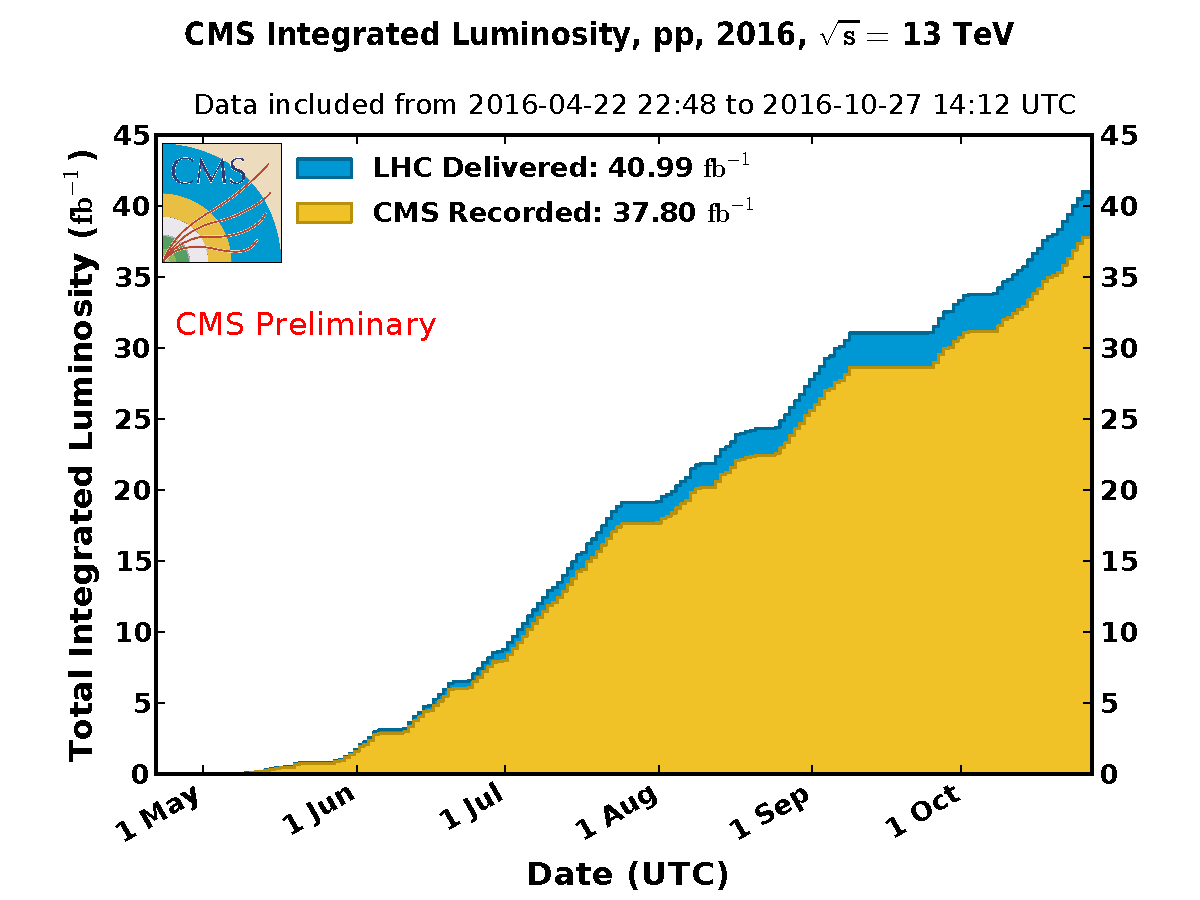
\includegraphics[width=.45\textwidth]{\PhDthesisdir/plots_and_images/from_CMS_lumi_public/lumi/int_lumi_per_day_cumulative_pp_2016.pdf}}
\hfill
\subcaptionbox{Distribution du nombre moyen d'interactions par croisement de faisceaux en 2016.\label{subfig-CMS_PU_profile_16}}[.45\textwidth]
{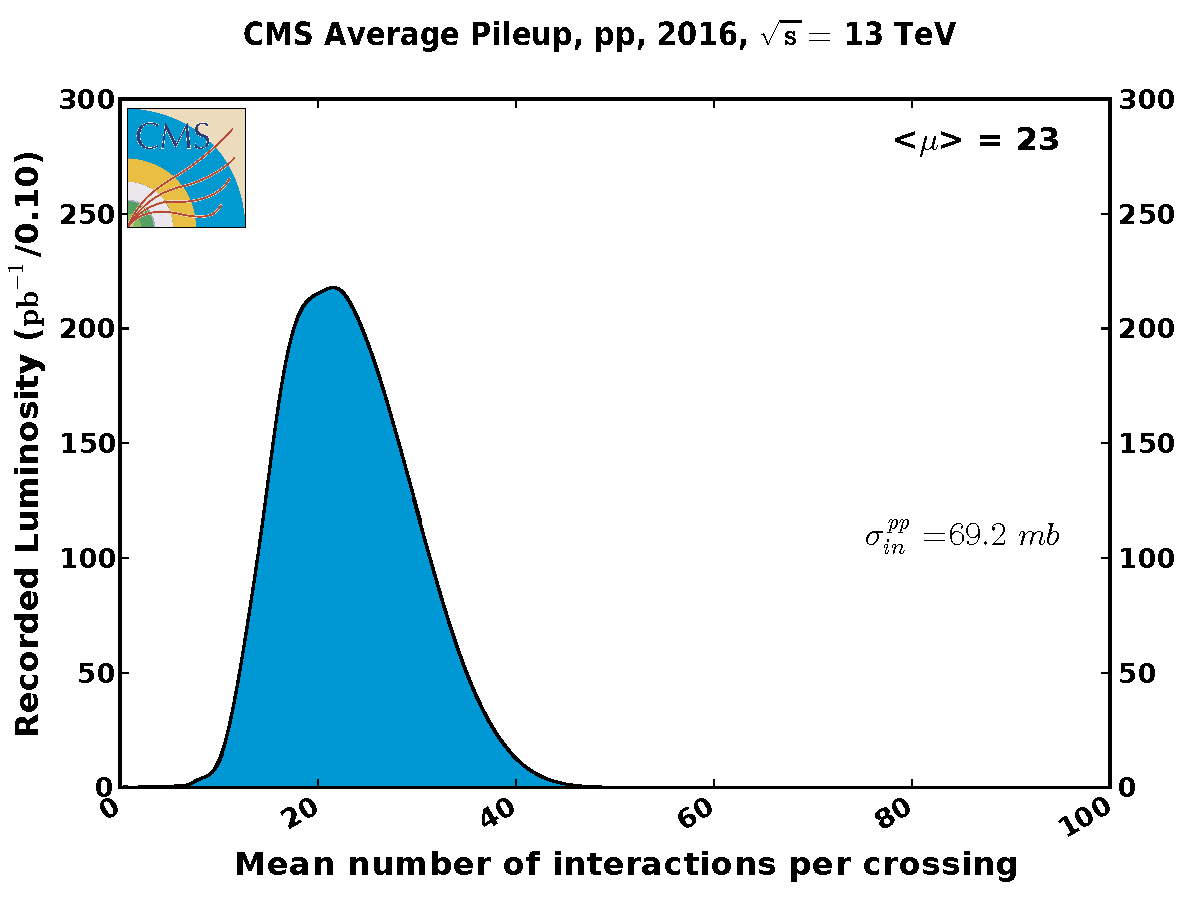
\includegraphics[width=.45\textwidth]{\PhDthesisdir/plots_and_images/from_CMS_lumi_public/PU/pileup_pp_2016_69200.pdf}}
\caption[Luminosité totale et empilement en 2016.]{Luminosité totale et empilement en 2016~\cite{CMS_lumi_public,CMS-PAS-LUM-17-001}.}
\label{fig-CMS_int_lumi_and_PU2016}

\vspace{.75\baselineskip}

\subcaptionbox{Luminosité totale délivrée par le LHC et enregistrée par le détecteur CMS en fonction du temps en 2017.\label{subfig-CMS_int_lumi_2017}}[.45\textwidth]
{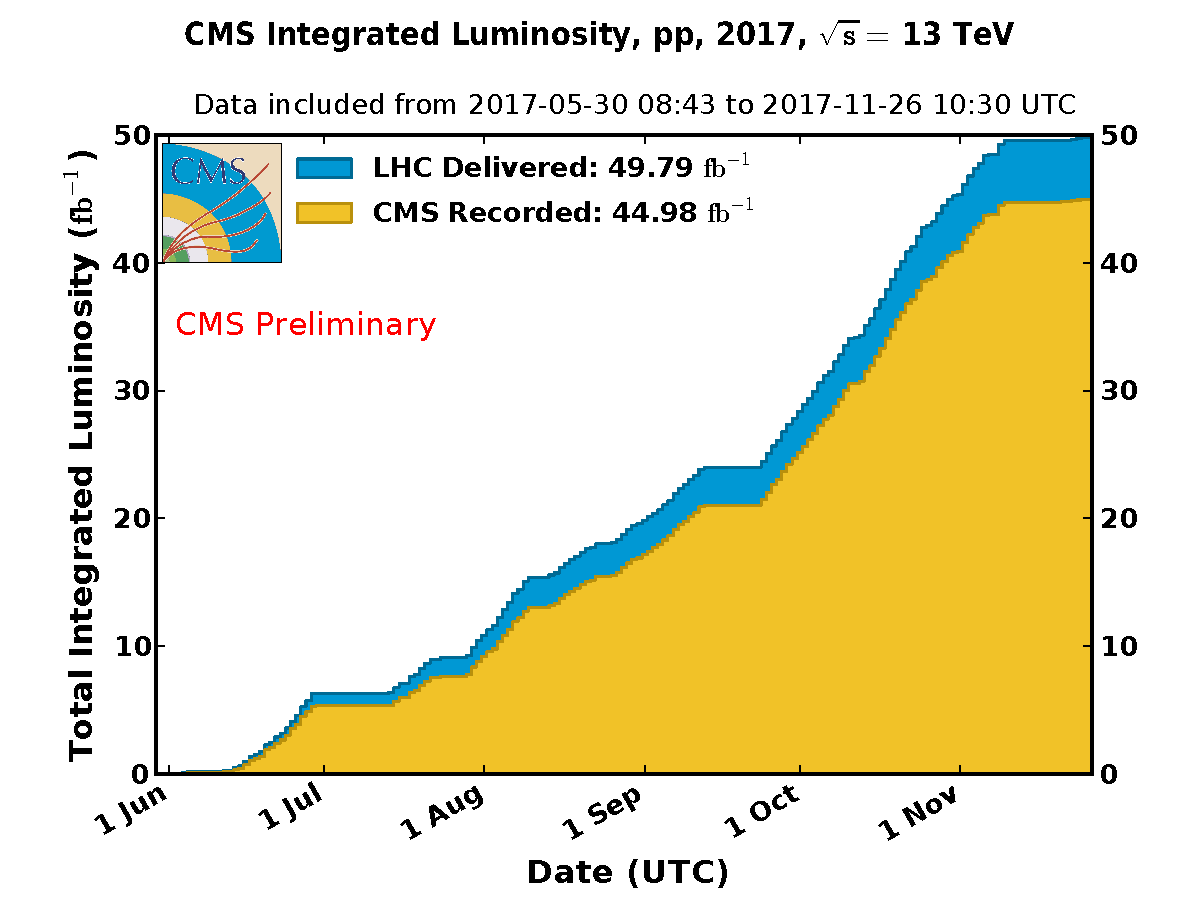
\includegraphics[width=.45\textwidth]{\PhDthesisdir/plots_and_images/from_CMS_lumi_public/lumi/int_lumi_per_day_cumulative_pp_2017NormtagLumi.pdf}}
\hfill
\subcaptionbox{Distribution du nombre moyen d'interactions par croisement de faisceaux en 2017.\label{subfig-CMS_PU_profile_17}}[.45\textwidth]
{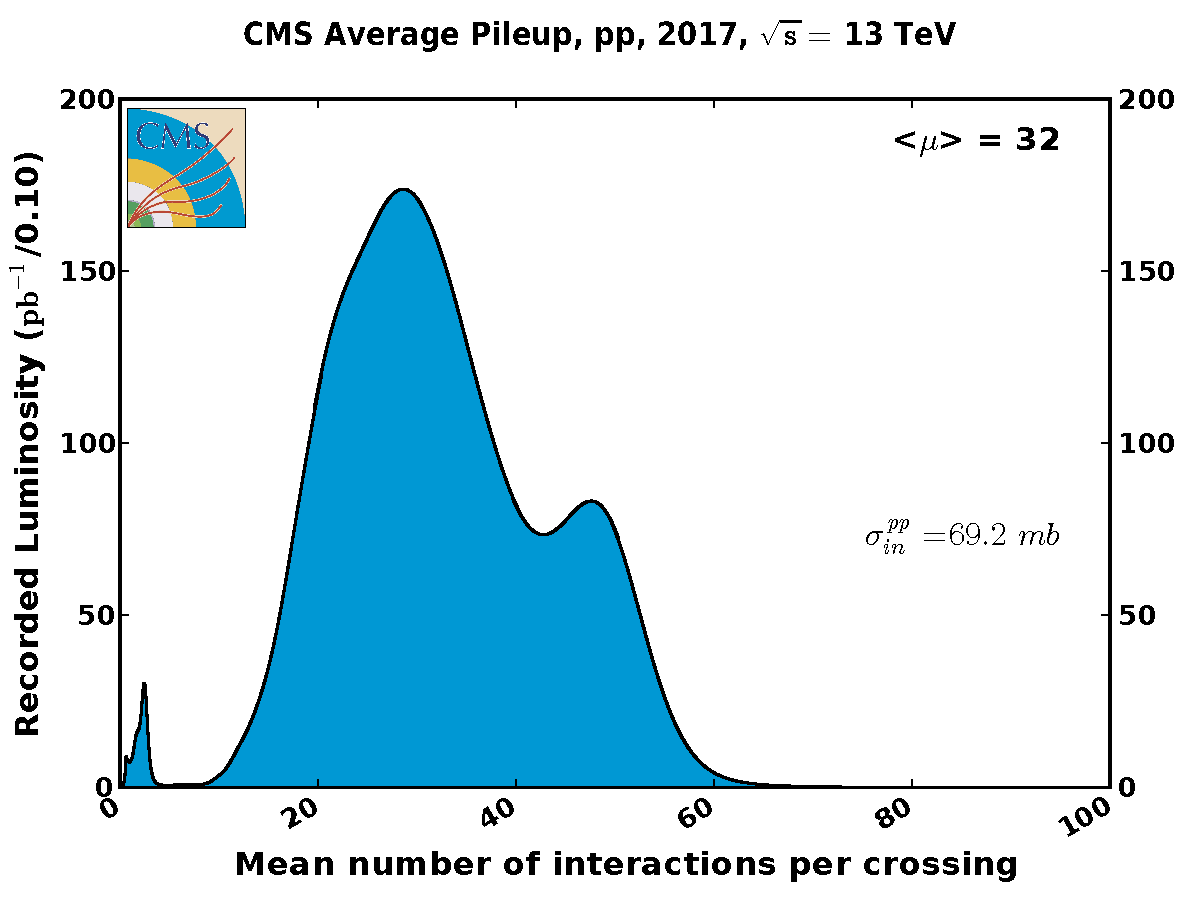
\includegraphics[width=.45\textwidth]{\PhDthesisdir/plots_and_images/from_CMS_lumi_public/PU/pileup_pp_2017_69200.pdf}}
\caption[Luminosité totale et empilement en 2017.]{Luminosité totale et empilement en 2017~\cite{CMS_lumi_public,CMS-PAS-LUM-17-004}.}
\label{fig-CMS_int_lumi_and_PU2017}

\vspace{.75\baselineskip}

\subcaptionbox{Luminosité totale délivrée par le LHC et enregistrée par le détecteur CMS en fonction du temps en 2018.\label{subfig-CMS_int_lumi_2018}}[.45\textwidth]
{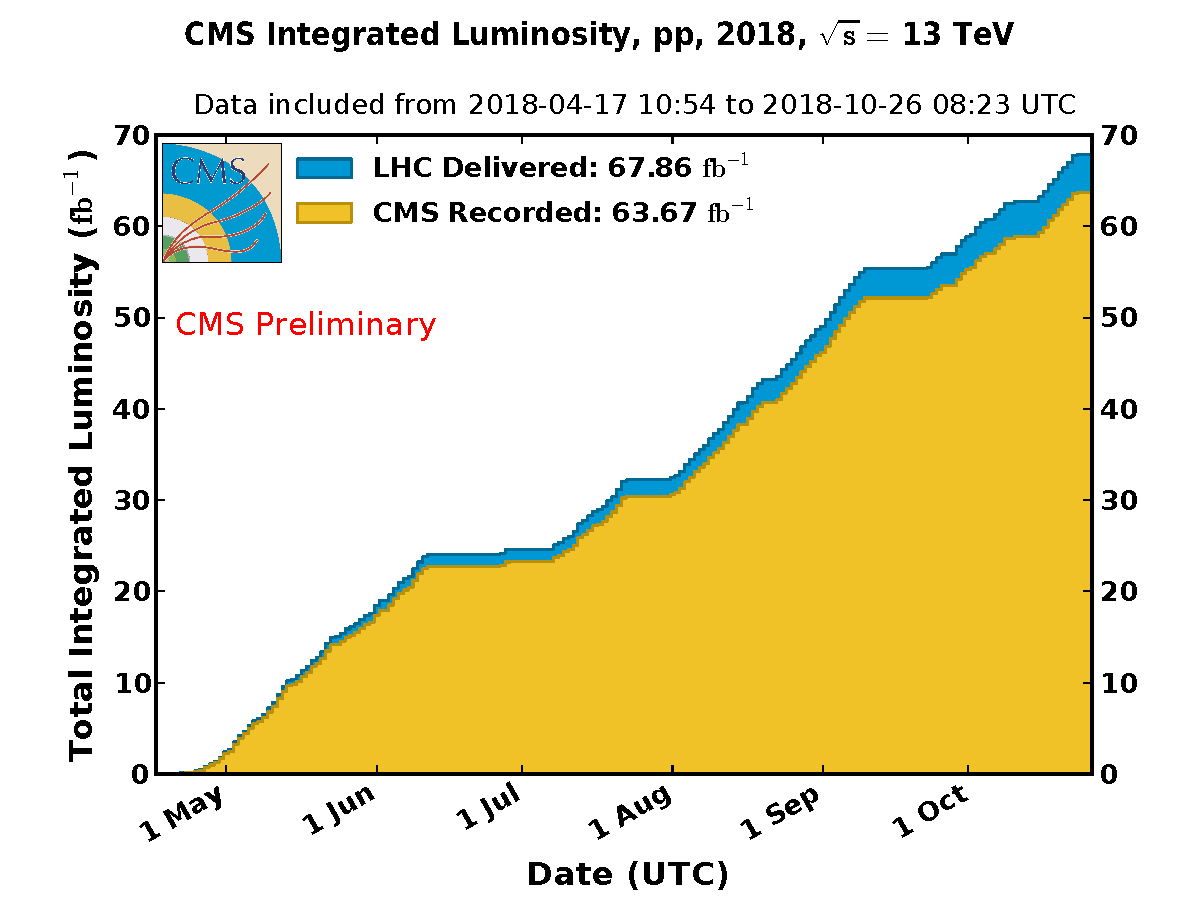
\includegraphics[width=.45\textwidth]{\PhDthesisdir/plots_and_images/from_CMS_lumi_public/lumi/int_lumi_per_day_cumulative_pp_2018NormtagLumi.pdf}}
\hfill
\subcaptionbox{Distribution du nombre moyen d'interactions par croisement de faisceaux en 2018.\label{subfig-CMS_PU_profile_18}}[.45\textwidth]
{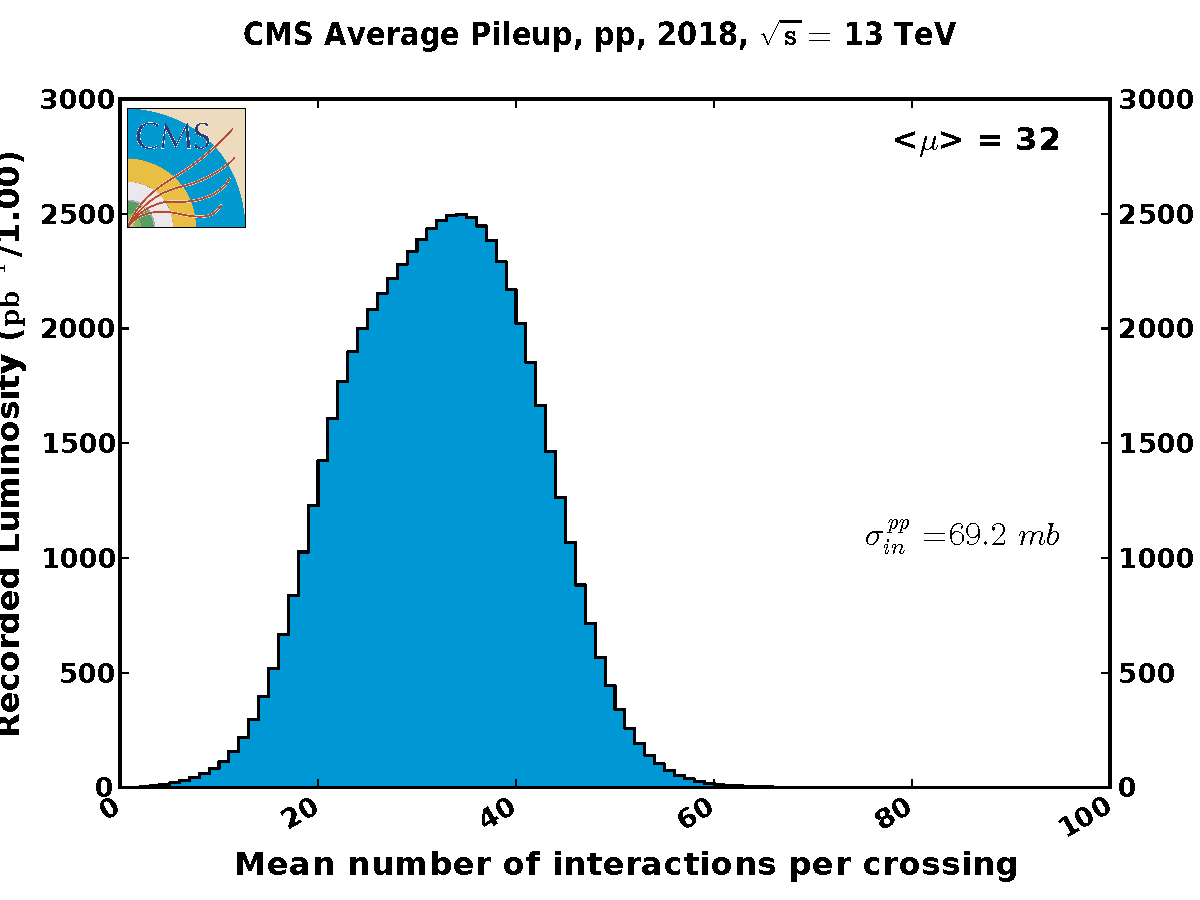
\includegraphics[width=.45\textwidth]{\PhDthesisdir/plots_and_images/from_CMS_lumi_public/PU/pileup_pp_2018_69200.pdf}}
\caption[Luminosité totale et empilement en 2018.]{Luminosité totale et empilement en 2018~\cite{CMS_lumi_public,CMS-PAS-LUM-18-002}.}
\label{fig-CMS_int_lumi_and_PU2018}
\end{figure}
\subsection{L'empilement}\label{chapter-LHC-section-LHC-subsec-PU}

\subsection{Les expériences du LHC}\label{chapter-LHC-section-LHC-subsec-experiments}
Il existe sept expériences au LHC.
Parmi elles, quatre sont de \og grandes expériences \fg{} et se situent chacune aux points d'interactions de l'anneau afin d'étudier les collisions qui y sont produites.
\begin{description}
\item[ALICE]\cite{alice_paper}, \emph{A Large Ion Collider Experiment}, est une expérience conçue pour étudier le déconfinement des quarks et des gluons à l'aide de collisions d'ions lourds. Ces études permettent de mieux comprendre le fonctionnement de la chromodynamique quantique ou QCD. Elle est installée au point~2 et réutilise l'aimant octogonal rouge très caractéristique de l'expérience L3 du LEP.
\item[ATLAS]\cite{atlas_paper}, \emph{A Toroidal LHC ApparatuS}, est une expérience généraliste avec un éventail d'études très large, allant des mesures de précision des paramètres du modèle standard à la recherche de nouvelle physique. Ce détecteur se trouve au point~1 du LHC.
\item[CMS]\cite{cms_paper}, \emph{Compact Muon Solenoid}, est également une expérience généraliste dont les objectifs sont similaires à ceux d'ATLAS. Les détecteurs d'ATLAS et de CMS étant conçus différemment, ces deux expériences peuvent valider leurs résultats de manière indépendante. Le détecteur CMS est installé au point~5 du LHC, à l'exact opposé d'ATLAS.
\item[LHCb]\cite{lhcb_paper}, \emph{Large Hadron Collider beauty}, se concentre sur l'étude de la violation de la symétrie $CP$ avec le quark~\quarkb, qui lui donne son nom. Cette expérience réalise également des mesures de précision de certains paramètres du modèle standard. L'expérience LHCb se situe au point~8.
\end{description}
\par Les trois autres expériences du LHC sont LHCf, TOTEM et MoEDAL.
L'expérience LHCf~\cite{lhcf_paper} (\emph{Large Hadron Collider forward}), installée à \SI{140}{\meter} de part et d'autre du détecteur ATLAS, observe les particules issues des collisions et presque alignées avec le faisceau du LHC afin de simuler des rayons cosmiques.
La plus \og longue \fg{} des expériences du CERN, TOTEM~\cite{totem_paper} (\emph{Total, elastic and diffractive cross-section measurement}), est quant à elle installée sur un demi kilomètre autour de CMS et étudie les protons grâce aux particules alignées avec le faisceau.
Enfin, MoEDAL~\cite{moedal_paper} (\emph{Monopole and Exotics Detector At the LHC}) cherche à détecter l'existence de monopoles magnétiques et de particules ionisantes massives prédites par certains modèles au-delà du modèle standard grâce à des détecteurs installés près de LHCb.